\documentclass[12pt]{article}

\usepackage[left=2.5cm,right=2.5cm,top=2.5cm,bottom=2.5cm]{geometry}
\usepackage{graphicx}
\usepackage[dvipsnames]{xcolor}
\usepackage{tikz}
\input{tikz/interfacepoint.tikzstyles}
\usepackage{tikz-cd}
\usepackage{tikz-qtree}
\usetikzlibrary{shapes,backgrounds,calc,arrows}
\usepackage{microtype}

\usepackage[setpagesize=false, colorlinks=true,urlcolor=red,pdftitle={Simplicial Coalgebras for Concurrent Regular Languages},pdfauthor={Hessel Sieburgh}]{hyperref}
\frenchspacing
\setlength\parindent{0pt}

\usepackage{amsmath}
\usepackage[utf8]{inputenc}
\usepackage{amsfonts}
\usepackage{amssymb}
\usepackage{amsthm}
\usepackage{theoremref}

\makeatletter
\renewcommand{\th@definition}{%
  \normalfont
  \thm@preskip 18pt \relax
  \thm@postskip 18pt \relax
}
\makeatother

\makeatletter
\renewcommand{\th@plain}{%
  \thm@preskip 18pt \relax
  \thm@postskip 18pt \relax
}
\makeatother

\newtheorem{theorem}{Theorem}[section]
\newtheorem{lemma}[theorem]{Lemma}
\newtheorem{corollary}[theorem]{Corollary}

\theoremstyle{definition}
\newtheorem{definition}[theorem]{Definition}
\newtheorem{example}[theorem]{Example}

\usepackage{bbm}
\usepackage{csquotes}
\usepackage{mathtools}
\usepackage{parskip}
\usepackage{mathtools}
\usepackage{mathdots}
%\usepackage[hidelinks]{hyperref}
\newcommand{\defeq}{\vcentcolon=}
\newcommand{\eqdef}{=\vcentcolon}

\DeclareMathOperator{\Ima}{Im}
\DeclareMathOperator{\sech}{sech}
\renewcommand{\P}{\mathcal{P}}
\newcommand{\R}{\mathbb{R}}
\newcommand{\C}{\mathbb{C}}
\newcommand{\N}{\mathbb{N}}
\newcommand{\E}[1]{\mathbb{E}\{#1\}}
\newcommand{\Q}{\mathbb Q}
\newcommand{\Z}{\mathbb{Z}}
\newcommand{\1}{\mathbbm{1}}
\newcommand{\ua}{\nearrow}
\newcommand{\da}{\searrow}
\newcommand{\eps}{\varepsilon}
\newcommand{\dx}{\mathrm{d}x}
\newcommand{\B}{\mathcal{B}}
\newcommand{\F}{\mathcal{F}}
\newcommand{\T}{\mathbb{T}}
\newcommand{\V}{\mathcal{V}}
\newcommand{\U}{\mathcal{U}}
\newcommand{\id}{\text{id}}
\newcommand{\I}{\mathcal{I}}
\newcommand{\A}{\mathcal{A}}
\newcommand{\J}{\mathcal{J}}
\newcommand{\G}{\mathcal{G}}
\renewcommand{\L}{\mathcal{L}}
\newcommand{\specepsilon}{\mathcal{E}}
\newcommand{\M}{\mathcal{M}}
\newcommand{\II}{\textbf{II}}
\newcommand{\bigo}{\mathcal{O}}
\renewcommand{\H}{\mathcal{H}}
\newcommand{\finP}{\mathcal{P}_{\omega}}
\newcommand{\Set}{\mathbf{Set}}

\begin{document}
\thispagestyle{empty}


\includegraphics{logoleiden}

\vspace{-2.5cm}\hfill \begin{huge}\textbf{Opleiding Informatica}\end{huge}

\vspace{5cm}
\begin{Large}
\hfill Simplicial Coalgebras

\vspace*{3mm}

\hfill for Concurrent Regular Languages

\vspace*{14mm}

\hfill Hessel Sieburgh
\end{Large}

\vspace*{6.0cm}

\begin{large}

Supervisors:\\
Henning Basold \& 
Marton Hablicsek


\vspace*{2.8cm}
BACHELOR THESIS

\vspace*{5mm}
Leiden Institute of Advanced Computer Science (LIACS)\\
\href{www.liacs.leidenuniv.nl}{\underline{\texttt{www.liacs.leidenuniv.nl}}}\hfill 01/07/2025
\end{large}

\newpage


\begin{abstract}
\noindent
This thesis introduces a construction of automata for concurrent languages. This is done by defining ranked hypergraphs, hypergraphs with interfaces that can be composed associatively. A simplicial set over these graphs is defined and we define F-coalgebras which give a nondeterministic transition model over the cells. The union of all paths of a tree resulting from a certain coalgebra gives a language of traces that support concurrent and sequential composition through the found operations on ranked hypergraphs. 
\end{abstract}

\bigskip

\thispagestyle{empty}
\tableofcontents
\thispagestyle{empty}

\clearpage
\setcounter{page}{1}

\section{Introduction} \label{introduction}

In this section we give an introduction to the problem addressed in this thesis.

% \begin{figure}
%     \centering
%     \begin{tikzpicture}
% 		\node [style={gra_point}, label={above:1}] (0) at (-1, 1.5) {};
% 		\node [style={gra_point}, label={above:2}] (1) at (-1, 0) {};
% 		\node [style={gra_point}, label={above:4}] (3) at (1, 1.5) {};
% 		\node [style={int_point}] (5) at (-3, 1.5) {};
% 		\node [style={int_point}] (6) at (-3, 0) {};
% 		\node [style={int_point}] (7) at (-3, -1.75) {};
% 		\node [style={int_point}] (8) at (3.75, 1.25) {};
% 		\node [style={int_point}] (9) at (3.75, -1.25) {};
% 		\node [style={gra_point}, label={above:6}] (10) at (1, -0.75) {};
% 		\node [style={gra_point}, label={above:5}] (11) at (1, 0.5) {};
% 		\node [label={above:a}] (12) at (0, 0) {};
% 		\node [label={above:b}] (13) at (0, 1.5) {};
% 		\node [style={gra_point}, label={above:3}] (14) at (0, -1.75) {};
% 		\draw [style={int_edge}] (5) to (0);
% 		\draw (1) to (12.center);
% 		\draw [style={int_edge}] (7) to (14);
% 		\draw [style={int_edge}] (6) to (1);
% 		\draw [style={int_edge}] (9) to (14);
% 		\draw [style={int_edge}] (9) to (10);
% 		\draw [style={int_edge}] (8) to (3);
% 		\draw [style={gra_edge}] (0) to (3);
% 		\draw [style={gra_edge}] (12.center) to (11);
% 		\draw [style={gra_edge}] (12.center) to (10);
%     \end{tikzpicture}
%     \caption{A Directed Acyclic (ranked) Hypergraph}
%     \label{fig:intro-DAH}
% \end{figure}


\subsection{The problem}

\subsection{Earlier research}

\subsection{Thesis overview}

\newpage
\section{Background}
\subsection{Presheaves}
\begin{definition}
    Let $C$,$D$ be categories, and $F,G: C\to D$ be functors. Then a \emph{natural transformation} $\mu: F\Rightarrow G$ from $F$ to $G$ is a family of morphisms such that:
    \begin{enumerate}
        \item for all $x\in C$ there exists a morphism $\mu_x: F(x)\to G(x)$ called the component at $x$
        \item for all $x,y\in C$ and all morphisms $f: x\to y$ the following diagram commutes:
        \begin{equation}\label{eq:nat-trans}
            \begin{tikzcd}
                F(x) \arrow{r}{F(f)} \arrow{d}{\mu_x} & F(y) \arrow{d}{\mu_y} \\
                G(x) \arrow{r}{G(f)} & G(y)
            \end{tikzcd}
        \end{equation}
    \end{enumerate}
\end{definition}

\begin{definition}
    Let $C$ be a category, a \emph{presheaf} is a functor \[
        F: C^{op}\to \Set
    \]
    The collection of all presheaves on a category forms a category with as morphisms the natural transformations between the presheaves.
\end{definition}

\subsection{Simplicial sets}
\begin{definition}
    The simplex category $\Delta$ has as objects
    \[
        [n] = \{0 < 1 < \dots < n\}
    \]
    and as morphisms the order-preserving functions between them.

    For all $n\in\N$, $i\in [n]$ we define the coface map $\delta^n_i: [n-1]\to [n]$ as the injective order preserving map which has $(\delta^n_i)^{-1}(i) = \varnothing$. So the map 'misses' $i$ and all other elements of $[n]$ are 'hit'.

    For all $n\in\N$, $i\in [n]$ we define the coface map $\sigma^n_i: [n-1]\to [n]$ as the surjective order preserving map which has $|(\sigma^n_i)^{-1}(i)| = 2$, $|(\sigma^n_i)^{-1}(j)| = 1$ $\forall j\neq i$. So the map 'hits' $i$ twice, and all other $j$ once.

    All morphisms of $\Delta$ are generated from the coface and codegeneracy maps.
\end{definition}

\textit{Notation: } $\delta_i^n$, $\sigma_i^n$ and so on, are just referred to as $\delta_i$, $\sigma_i$ etc. As the exact $n$ is not necessary for most applications. 

\begin{definition}
    A \emph{simplicial set} is a presheaf on \( \Delta \), which means a simplicial set is a functor
    \[
    X \colon \Delta^{\mathrm{op}} \to \Set
    \]
    
    Thus, a simplicial set \( X \) assigns to each \( [n] \in \Delta \) a set \( X_n = X([n]) \) of \emph{n-simplices}, and to each morphism \( \theta \colon [m] \to [n] \), a function \( X(\theta) \colon X_n \to X_m \).
    
    In particular, we have $X(\delta_i) = d_i$ where $d_i: X_n\to X_{n-1}$ omits the $i$-th element from an $n$-simplex. And $X(\sigma_i) = s_i$ where $s_i: X_n \to X_{n+1}$ repeats the $i$-th element in the simplex.
    
    These satisfy the \emph{simplicial identities}:
    \[
    \begin{aligned}
    d_i d_j &= d_{j-1} d_i && \text{if } i < j, \\
    s_i s_j &= s_{j+1} s_i && \text{if } i \leq j, \\
    d_i s_j &=
    \begin{cases}
    s_{j-1} d_i & \text{if } i < j, \\
    \mathrm{id} & \text{if } i = j \text{ or } i = j+1, \\
    s_j d_{i-1} & \text{if } i > j+1.
    \end{cases}
    \end{aligned}
    \]

    The presheaf category of simplicial sets is called $\mathrm{sSet}$ and its natural transformations the \emph{simplicial morphisms}.
    
    Given a collection of sets $S = S_0 \sqcup S_1 \sqcup \dots$ and functions $d_i: S_n\to S_{n-1}$, $s_i: S_n \to S_{n+1}$ satisfying the simplicial identities there is a unique simplicial set which has the same face and degeneracy maps.
\end{definition}

\begin{lemma}
    Let $X, Y\in \mathrm{sSet}$, a collection of morphisms $f_0: X_0\to Y_0, f_1: X_1\to Y_1, \dots$ is a simplicial morphism if and only if the following diagrams commute.
    \[
        \begin{tikzcd}
        X_n \arrow{r}{d_i^X} \arrow{d}{f_n} & X_{n-1} \arrow{d}{f_{n-1}} \\
        Y_n \arrow{r}{d_i^Y} & Y_{n-1}
        \end{tikzcd}
        \quad
        \begin{tikzcd}
        X \arrow{r}{s_j^X} \arrow{d}{f_n} & X_{n+1} \arrow{d}{f_{n+1}} \\
        Y_n \arrow{r}{s_j^Y} & Y_{n+1}
        \end{tikzcd}
    \]
\end{lemma}

\begin{proof}
    Given that $\delta_i$, $\sigma_i$ generate the morphisms in $\Delta$, diagram \ref{eq:nat-trans} automatically commutes for all $f$ if it does so for $\delta$ and $\sigma$.
\end{proof}
\subsection{Subobject Classifiers}
\begin{definition}
    Let $f, g$ be morphisms defined by
    \begin{center}
        \begin{tikzcd}
              & Y \arrow[d,"g"] \\
              X \arrow[r,swap,"f"]  & Z
        \end{tikzcd}
    \end{center}

    Then a \emph{pullback} is an object $P$ together with morphisms $p_1, p_2$ such that 
    \begin{center}
        \begin{tikzcd}
            P \arrow[d,"p_1"] \arrow[r,"p_2"] & Y \arrow[d,"g"] \\
            X \arrow[r,swap,"f"]  & Z
        \end{tikzcd}
    \end{center}
    commutes and is universal. The universal property means that for any other object $Q$, with morphisms $q_1: Q\to X$, $q_2: Q\to Y$ such that they commute just like the above, there needs to be a morphism $\beta: Q\to P$ such that this whole diagram commutes. 

    \begin{center}
        \begin{tikzcd}
            Q \arrow[rrd,bend left,"q_2"]
                \arrow[ddr,bend right,swap,"q_1"]
                \arrow[dr,dashed,"\beta"] \\
            & P \arrow[d,"p_1"] \arrow[r,"p_2"] & Y \arrow[d,"g"] \\
            & X \arrow[r,swap,"f"]  & Z
        \end{tikzcd}
    \end{center}
\end{definition}

\begin{definition}
    Let $C$ be a category with a terminal object $*$ and finite limits. A \emph{subobject classifier} $\Omega$ is an object in $C$ such that there exists a morphism $\top: * \to \Omega$ which has the property that for all objects $A, X$ and monomorphisms $f: A\to X$ there exists a unique morphism $\chi_A: X\to \Omega$ that makes the diagram commute and be a pullback
    \begin{center}
        \begin{tikzcd}
            A \arrow[d,"f"] \arrow[r,""] & * \arrow[d,"\top"] \\
            X \arrow[r,"\chi_A"] & \Omega
        \end{tikzcd}
    \end{center}
\end{definition}

\begin{example}
    In the category $\mathrm{Set}$ where objects are sets and morphisms are functions, the subobject classifier is $\Omega = \{0,1\}$ and if $f = \id$ then $\chi_A$ is the characteristic map of the subset $A\subseteq X$.
\end{example}

\begin{lemma}[{\cite[Lemma.~1.6.5]{Elephant}}]\label{lem:exist-sub_class}
    For any small category $C$, the functor category $[C, \mathrm{Set}]$ has a subobject classifier.
\end{lemma}

\begin{corollary}
    $\mathrm{sSet}$ has a subobject classifier $\Omega$.
\end{corollary}

\begin{proof}
    Given a category $C$ the presheaf category is the same as the functor category $[C^{op}, \mathrm{Set}]$. $\Delta$ is a small category (we won't go into detail in this detail what constitutes as a small category), and therefore so is its dual. From \ref{lem:exist-sub_class} we find that $\mathrm{sSet} = [\Delta^{op}, \mathrm{Set}]$ has a subobject classifier $\Omega$.
\end{proof}

\subsection{Coalgebras}
In this thesis we primarily work with $F$-coalgebras, which we will introduce next, these are a special type of coalgebra which fits our usecase very well. A general definition therefore is not necessary as the definition of $F$-coalgebras is self-contained.

\begin{definition}
    Given a category $C$ and an endofunctor $F: C \to C$. An $F$-coalgebra $(A,\alpha)$ is an object $A\in C$ called the carrier and a morphism $\alpha: A\to FA$.
\end{definition}

\begin{example}[Labelled transition systems]
    A very illustrative example are labelled transition systems. Here we have as carrier a state space $X$, and a set of actions (or characters in the context of DFA) $A$.

    Take as endofunctor 
    \[
        FX = \P(A\times X)
    \]

    Then given a state $x\in X$, $\alpha(x) = \{(a_1, x_1),(a_2, x_2), \dots\}$ denotes possible transitions to states $x_1, x_2, \dots$ with corresponding outputs of $a_1, a_2, \dots$.
    \begin{figure}[h]
        \centering
        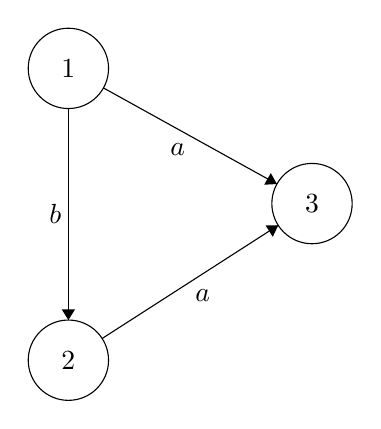
\begin{tikzpicture}[scale=0.17]
            \tikzstyle{every node}+=[inner sep=0pt]
            \draw [black] (17.2,-13.3) circle (3);
            \draw (17.2,-13.3) node {$1$};
            \draw [black] (17.2,-35.1) circle (3);
            \draw (17.2,-35.1) node {$2$};
            \draw [black] (35.4,-23.4) circle (3);
            \draw (35.4,-23.4) node {$3$};
            \draw [black] (19.82,-14.76) -- (32.78,-21.94);
            \fill [black] (32.78,-21.94) -- (32.32,-21.12) -- (31.83,-21.99);
            \draw (25.36,-18.85) node [below] {$a$};
            \draw [black] (17.2,-16.3) -- (17.2,-32.1);
            \fill [black] (17.2,-32.1) -- (17.7,-31.3) -- (16.7,-31.3);
            \draw (16.7,-24.2) node [left] {$b$};
            \draw [black] (19.72,-33.48) -- (32.88,-25.02);
            \fill [black] (32.88,-25.02) -- (31.93,-25.03) -- (32.47,-25.88);
            \draw (27.24,-29.75) node [below] {$a$};
        \end{tikzpicture}
        \label{ex-lab_tran_sys}
        \caption{A labelled transition system}
    \end{figure}

    In figure \ref{ex-lab_tran_sys} a labelled transition system is given where $\alpha(1) = \{(a,3),(b,2)\}$, $\alpha(2) = \{(a,3)\}$, $\alpha(3) = \varnothing$.
\end{example}

\newpage
\section{Definitions}
\subsection{Ranked Hypergraphs}
\begin{definition}
    A directed \emph{hypergraph} $(V,H)$ is a finite set of vertices $V$ and a set of \emph{hyperarcs} $H\subseteq \P(V)^2$.
\end{definition}

\emph{Notation:} A directed hypergraph containing no cycles is a Directed Acyclic Hypergraph (DAH).

\begin{definition}
A \emph{ranked term hypergraph} $(g, r, o, \L, A)$ consists of:
\begin{itemize}
\item A DAH $g$,
\item Finite sequences $r = (r_i)_i$, $o = (o_i)_i$ $r_i, o_i\in \P(V)$ denoting the root and variable interfaces. $o_i$ contains only maximal vertices. We refer to $(|r|, |o|)$ as the \emph{rank} of this graph.
\item An action set $A$ and a hyperarc labelling function $\L: H\to A$
\end{itemize}
\end{definition}
\emph{Notation:} In this thesis we refer to ranked term hypergraphs as just hypergraphs as we will only be working with this kind. $HG(n,m)$ is the set of ranked term  hypergraphs of rank $(n,m)$

A ranked hypergraph with $|r| = |o|$ is called symmetric.

\begin{example}
    In figure \ref{fig:DAH-example} a ranked hypergraph is drawn. Left is the root interface, of rank 3, on the right is the output interface of rank 2. 

    The full definition of this graph is as follows
    \begin{itemize}
        \item $V = \{1,2,3,4,5,6\}$
        \item $H = \{(\{1\}, \{4\}), (\{2\}, \{5,6\})\}$
        \item $r = (\{1\}, \{2\}, \{3\})$, $o = (\{4\}, \{3,6\})$
        \item $A = \{a,b\}$, $\L((\{1\}, \{4\})) = b$, $\L((\{2\}, \{5,6\})) = a$
    \end{itemize}
    
    \begin{figure}[h]
    \centering
    \begin{tikzpicture}
		\node [style={gra_point}, label={above:1}] (0) at (-1, 1.5) {};
		\node [style={gra_point}, label={above:2}] (1) at (-1, 0) {};
		\node [style={gra_point}, label={above:4}] (3) at (1, 1.5) {};
		\node [style={int_point}] (5) at (-3, 1.5) {};
		\node [style={int_point}] (6) at (-3, 0) {};
		\node [style={int_point}] (7) at (-3, -1.75) {};
		\node [style={int_point}] (8) at (3.75, 1.25) {};
		\node [style={int_point}] (9) at (3.75, -1.25) {};
		\node [style={gra_point}, label={above:6}] (10) at (1, -0.75) {};
		\node [style={gra_point}, label={above:5}] (11) at (1, 0.5) {};
		\node [label={above:a}] (12) at (0, 0) {};
		\node [label={above:b}] (13) at (0, 1.5) {};
		\node [style={gra_point}, label={above:3}] (14) at (0, -1.75) {};
		\draw [style={int_edge}] (5) to (0);
		\draw (1) to (12.center);
		\draw [style={int_edge}] (7) to (14);
		\draw [style={int_edge}] (6) to (1);
		\draw [style={int_edge}] (9) to (14);
		\draw [style={int_edge}] (9) to (10);
		\draw [style={int_edge}] (8) to (3);
		\draw [style={gra_edge}] (0) to (3);
		\draw [style={gra_edge}] (12.center) to (11);
		\draw [style={gra_edge}] (12.center) to (10);
    \end{tikzpicture}
    \caption{A Directed Acyclic Hypergraph}
    \label{fig:DAH-example}
\end{figure}
\end{example}


\subsection{Composition of ranked hypergraphs}
\begin{definition}\label{def_seq_comp}
Let $G, F$ be hypergraphs such that $|o^G| = |r^F|$, their composition is defined as follows:
\begin{align}
    G\otimes F = (g', r', o^F, \L^G\sqcup \L^F, A^G\cup A^F)
\end{align}

We obtain $g' = (V,H)$ by the following procedure:

Define 
% \begin{enumerate}
%     \item $g' = (V,H) \defeq g^G \sqcup g^F$
%     \item For each $o^G_i\in o^G$, $v\in o^G_i$, if v is minimal and/or $r^F_i\neq\varnothing$:\\ $V\defeq V\setminus \{v\}$ and for each $(U, U')\in H$ with $v\in U'$, set $U' \defeq (U' \cup r^F_i) \setminus \{v\}$\\
% \end{enumerate}

\begin{align*}
    V = (V^G + V^F) \setminus \bigcup_{i\leq |o^G|}o^G_i
\end{align*}

To get the hyperarcs we keep all elements but replace a vertex if it exists in an output, to do this neatly we define a pair of functions:

\[
\psi_{r^F, o^G}(v) := 
\begin{cases}
\displaystyle\bigcup_{\substack{i\leq |o^G| \\ v \in o^G_i}} r^F_i & \text{if } \exists i \leq |o^G| \text{ such that } v \in o^G_i \\
\{v\} & \text{otherwise}
\end{cases}
\]

\[
\Psi_{r^F, o^G}(U') := \bigcup_{v \in U'} \psi_{r^F, o^G}(v)
\]

\[
H := \left\{ \left(U, \Psi_{r^F, o^G}(U')\right) : (U, U') \in H^G \right\} \cup H^F
\]

So for all $i$, in each arc $v$ that ends in a vertex in $o_i^G$, we replace that vertex in the arc with $r_i^F$. 

And we obtain $r'$ by taking over the original $r^G$ and `connecting through' for vertices which are both minimal and maximal:
\begin{align*}
    r'_i = \Psi_{r^F, o^G}(r^G_i)
\end{align*}
\end{definition}

This composition allows for a left identity $id_n$ namely $id_n = ((\{1,2,\dots,n\}, \varnothing), (\{i\})_{i\in n}, (\{i\})_{i\in n})$.\vspace{5pt}

\begin{lemma}\label{lem:psieq}
    Let $G,K,F$ be a DAH and $U\subseteq V^G$ a set of vertices. It holds that:
    \[
        \Psi_{r^F, o^K}\circ \Psi_{r^K, o^G}(U) = \Psi_{r^F\otimes r^K, o^G}(U)
    \]
\end{lemma}

\begin{proof}
    We prove the lemma for a singleton, this then extends trivially to all subsets $U\subseteq V^G$. Let $v\in V^G$, we proceed by using the definitions:
    \begin{align*}
        \Psi_{r^F, o^K}\circ \psi_{r^K, o^G}(v) &= 
        \begin{cases}
            \{v\} & v\notin \cup_i o_i^G\\
            \Psi_{r^F, o^K}\left(\bigcup_{\substack{i \leq |r^K| \\ v \in o^G_i}} r^K_i\right) & \text{else}
        \end{cases}\\
        \intertext{Because both unions are finite we can exchange them: }
        &= 
        \begin{cases}
            \{v\} & v\notin \cup_i o_i^G\\
            \bigcup_{\substack{i \leq |r^K| \\ v \in o^G_i}} \Psi_{r^F, o^K} (r^K_i) & \text{else}\\
        \end{cases}\\
        \intertext{By definition $r^{K\otimes F}_i \defeq \Psi_{r^F, o^K} (r^K_i)$ and hence}
        &=
        \begin{cases}
            \{v\} & v\notin \cup_i o_i^G\\
            \bigcup_{\substack{i\leq  |r^{K\otimes F}| \\ v \in o^G_i}} r^{K\otimes F}_i & \text{else}\\
        \end{cases}\\
        &= \psi_{r^F\otimes r^K, o^G}(v)
    \end{align*}

    Taking unions of singletons then yields:
    \[
        \Psi_{r^F, o^K}\circ \Psi_{r^K, o^G}(U) = \Psi_{r^F\otimes r^K, o^G}(U)
    \]
\end{proof}

Which lets us prove the following theorem:

\begin{theorem}\label{thm:assoc}
The sequential composition of ranked hypergraphs has the following properties:
    \begin{enumerate}
        \item $\otimes$ is associative
        \item $id_n \otimes G = G$
    \end{enumerate}
\end{theorem}

\begin{proof}
    Let $G,K,F$ be ranked hypergraphs. It is clear from the definition that $(G \otimes K) \otimes F = G \otimes (K \otimes F)$ if and only if their graphs and root interfaces are equal.
         
    Let $r$, $r'$ be the root interfaces for $(G \otimes K) \otimes F$, $G \otimes (K \otimes F)$ respectively.  
    We expand the definition and use lemma \ref{lem:psieq} to show that $r = r'$. Let $i\leq |r^G|$, we get:
    
    \begin{align*}
        r_i = \Psi_{r^F, o^k}(r^{G\otimes K}_i) = \Psi_{r^F, o^k}(\Psi_{r^K, o^G}(r^G_i)) = \Psi_{r^{K\otimes F}, o^G}(r_i) = r'_i\\
    \end{align*}

    Let $g = (V, H)$, $g' = (V', H')$ be the graphs for $(G \otimes K) \otimes F$, $G \otimes (K \otimes F)$ respectively.

    We expand the definition:
    \begin{gather*}
        V = (V^{G\otimes K} + V^F) \setminus \bigcup_{i\leq |o^K|}o_i^K\\
        = (((V^G + V^K) \setminus \bigcup_{i\leq|o^G|}o^G_i) + V^F) \setminus \bigcup_{i\leq |o^K|}o_i^K
        \intertext{From disjointness the inclusion of $V^G$, $V^K$, and $V^F$ into their coproduct we get}
        = (V^G + ((V^K + V^F) \setminus \bigcup_{i\leq|o^K|}o^K_i)) \setminus \bigcup_{i\leq|o^G|}o_i^G = V'
    \end{gather*}

    Lastly for the arcs:
    \begin{align*}
        H &= \left\{ \left(U, \Psi_{r^F, o^K}(U')\right) : (U, U') \in H^{G\otimes K} \right\} \cup H^F\\
        &= \left\{ \left(U, \Psi_{r^F, o^K}(\Psi_{r^K, o^G}(U'))\right) : (U, U') \in H^G \right\}
        \cup \left\{ \left(U, \Psi_{r^F, o^K}(U')\right) : (U, U') \in H^K \right\} \cup H^F\\
        \intertext{By lemma \ref{lem:psieq} we have}
        &= \left\{ \left(U, \Psi_{r^{F\otimes K}, o^G}(U')\right) : (U, U') \in H^G \right\}
        \cup \left\{ \left(U, \Psi_{r^F, o^K}(U')\right) : (U, U') \in H^K \right\} \cup H^F\\
        &= \left\{ \left(U, \Psi_{r^{K \otimes F}, o^G}(U')\right) : (U, U') \in H^G \right\} \cup H^{K \otimes F}\\
        &= H'
    \end{align*}
\end{proof}

\begin{theorem}
    The set of ranked hypergraphs is generated by the subset of hypergraphs $HG_0$ with depth of at most 1. 
\end{theorem}

\begin{proof}
    We prove this by showing that for any hypergraph $G$ of depth $\geq 2$ there exist hypergraphs $G_{start}\in HG$, $G_{end}\in HG_0$ such that $G = K\otimes F$.

    First take $r^{start} = r$, $o^{end} = o$, $\L_{start} = \L_{end} = \L$, $A_{start} = A_{end} = A$.

    Let $n$ be the depth of the graph, and denote by $d: V\to \N$ the depth of a vertex.

    Pull apart the vertices into two sets, which only coincide at depth $n-1$:
    \begin{align*}
        &V_{start} = \{v\in V : d(v) \neq n \}\\
        &V_{end} = \{v\in V : d(v) \in \{n - 1, n\} \} \cup \bigcup_{i\leq |o|} o_i
    \end{align*}

    this also adds dummy vertices to $G_{end}$ for vertices of depth $< n-1$ which are in some output interface.

    Then let:
    \begin{align*}
        &H_{end} = \{(U,U')\in H : d(v) = n\quad\forall v\in U'\}\\
        &H_{start} = \{(U,U')\in H : d(v) < n\quad\forall v\in U'\}
    \end{align*}

    Note that for all $(U,U')\in H$ there exists a $k\in \N$ such that for all $v\in U'$ we have $d(v) = k$.

    Finally for the interfaces, take $r_{end} = o_{start}$ to be any enumeration of all elements of $V_{start}\cap V_{end}$.

    We work out $G_{start};G_{end}$
\end{proof}

\begin{definition}
    Let $G,F$ be hypergraphs such that $|o^G| \leq |r^F|$ we extend the notion of the sequential composition given by \ref{def_seq_comp} to asymmetric graph compositions. Write 

    \begin{align*}
        G\otimes^+ F = (g', r', o^F, \L^G\sqcup \L^F, A^G\cup A^F)
    \end{align*}

    for the extended composition.

    We obtain $g' = (V,H)$ by the following procedure:

    \[
        V \defeq (V^G + V^F) \setminus \bigcup_{i\leq |o^G|}o^G_i    
    \]
    
    \[
        H \defeq \left\{ \left(U, \Psi_{r^F, o^G}(U')\right) : (U, U') \in H^G \right\} \cup H^F
    \]

    And do the same as $\otimes$ for the interfaces except for the excess ones which we just copy:
    \[
        r'_i = 
        \begin{cases}
            \Psi_{r^F, o^G}(r^G_i) & i\leq |o^G|\\
            r^F_i & else
        \end{cases}
    \]
\end{definition}

By separation of cases we trivially extend theorem \ref{thm:assoc} to the following result:
\begin{corollary}
    $\otimes^+$ is associative
\end{corollary}

\subsection{Simplicial set over ranked term graphs}
\begin{definition}
    Let $V$ be the vertex set of a ranked hypergraph.\\
    We define the monoid $\M = (\P(V)^2, (\varnothing, \varnothing), \cup\times\cup)$. 
\end{definition}

From this monoid we define a simplicial set using the nerve construction.

\begin{definition}
    The \emph{nerve} $N(\M)$ of the monoid $\M$ is the simplicial set where:
    \begin{align*}
        N(\M)_n = \M^n\\
        d^{\M}_i(m_1,\dots,m_n) = 
        \begin{cases}
            (m_1,\dots,m_i \cup\times\cup m_{i+1}, \dots, m_n) & 0 < i < n\\
            (m_2,\dots, m_n) & i = 0\\
            (m_1,\dots,m_{n-1}) & i = n
        \end{cases}\\
        s^{\M}_i(m_1,\dots,m_n) = (m_1, \dots, m_i, (\varnothing, \varnothing), m_{i+1}, \dots, m_n)\\
    \end{align*}
\end{definition}

\begin{definition}
Define the simplicial set $\H$ by $\H_n = HG(n,n)$. And the face and degeneracy maps:
\begin{align*}
    &d_i^{\H} ((g, (U_1, \dots, U_n), (W_1, W_2, \dots, W_n), \L, A))\\
    &\quad=\begin{cases}
        (g, (U_1, \dots, U_i\cup U_{i+1}, \dots U_n), (W_1, \dots, W_i\cup W_{i+1}, \dots W_n), \L, A) & 0 < i < n\\
        (g, (U_2, \dots, U_n), (W_1, W_2, \dots, W_n), \L, A) & i = 0\\
        (g, (U_1, \dots, U_{n-1}), (W_1, \dots, W_{n-1}), \L, A) & i = n
    \end{cases}\\
    \hspace{5pt}
    &s_i^{\H}((g, (U_1, \dots, U_n), (W_1, W_2, \dots, W_n), \L, A))\\
    &=\quad (g, (U_1, \dots U_i, \varnothing, U_{i+1}, \dots, U_n), (W_1, \dots W_i, \varnothing, W_{i+1}, \dots, W_n), \L, A)
\end{align*}
\end{definition}

\begin{lemma}
    $\H$ is indeed a simplicial set.
\end{lemma}

\begin{proof}
    Let $\pi_n: \H_n \to N(\M)_n$ be the projection onto the interfaces given by $\pi_n((g, r, o, \L, A)) = ((r_i, o_i))_{i\in [n]}$.

    \emph{Claim: } the following diagrams commute.
    \[
    \begin{tikzcd}
    \H_n \arrow{r}{d_i^{\H}} \arrow{d}{\pi_n} & \H_{n-1} \arrow{d}{\pi_{n-1}} \\
    N(\M)_n \arrow{r}{d_i^\M} & N(\M)_{n-1}
    \end{tikzcd}
    \quad
    \begin{tikzcd}
    \H_n \arrow{r}{s_j^{\H}} \arrow{d}{\pi_n} & \H_{n+1} \arrow{d}{\pi_{n+1}} \\
    N(\M)_n \arrow{r}{s_j^\M} & N(\M)_{n+1}
    \end{tikzcd}
    \]
    \begin{align*}
        \intertext{\textbf{Face maps}\\$i = 0$:}
        &\pi_{n-1}(d_0^\mathcal{H}((g, (U_1, \ldots, U_n), (W_1, \ldots, W_n), \mathcal{L}, A))) \\
        &= \pi_{n-1}((g, (U_2, \ldots, U_n), (W_2, \ldots, W_n), \mathcal{L}, A)) \\
        &= ((U_2, W_2), \ldots, (U_n, W_n)) \\
        &= d_0^\mathcal{M}((U_1, W_1), \ldots, (U_n, W_n)) \\
        &= d_0^\mathcal{M}(\pi_n((g, (U_1, \ldots, U_n), (W_1, \ldots, W_n), \mathcal{L}, A))) \\
        \intertext{$0 < i < n$:}
        &\pi_{n-1}(d_i^\mathcal{H}((g, (U_1, \ldots, U_n), (W_1, \ldots, W_n), \mathcal{L}, A))) \\
        &= \pi_{n-1}((g, (U_1, \ldots, U_i \cup U_{i+1}, \ldots, U_n), (W_1, \ldots, W_i \cup W_{i+1}, \ldots, W_n), \mathcal{L}, A)) \\
        &= ((U_1, W_1), \ldots, (U_i \cup U_{i+1}, W_i \cup W_{i+1}), \ldots, (U_n, W_n)) \\
        &= d_i^\mathcal{M}((U_1, W_1), \ldots, (U_n, W_n)) \\
        &= d_i^\mathcal{M}(\pi_n((g, (U_1, \ldots, U_n), (W_1, \ldots, W_n), \mathcal{L}, A))) \\
        \intertext{$i = n$:}
        &\pi_{n-1}(d_n^\mathcal{H}((g, (U_1, \ldots, U_n), (W_1, \ldots, W_n), \mathcal{L}, A))) \\
        &= \pi_{n-1}((g, (U_1, \ldots, U_{n-1}), (W_1, \ldots, W_{n-1}), \mathcal{L}, A)) \\
        &= ((U_1, W_1), \ldots, (U_{n-1}, W_{n-1})) \\
        &= d_n^\mathcal{M}((U_1, W_1), \ldots, (U_n, W_n)) \\
        &= d_n^\mathcal{M}(\pi_n((g, (U_1, \ldots, U_n), (W_1, \ldots, W_n), \mathcal{L}, A)))\\
        \intertext{\textbf{Degeneracy maps}}
        &\pi_{n+1}(s_i^\mathcal{H}((g, (U_1, \ldots, U_n), (W_1, \ldots, W_n), \mathcal{L}, A))) \\
        &= \pi_{n+1}((g, (U_1, \ldots, U_i, \varnothing, U_{i+1}, \ldots, U_n), (W_1, \ldots, W_i, \varnothing, W_{i+1}, \ldots, W_n), \mathcal{L}, A)) \\
        &= ((U_1, W_1), \ldots, (U_i, W_i), (\varnothing, \varnothing), (U_{i+1}, W_{i+1}), \ldots, (U_n, W_n)) \\
        &= s_i^\mathcal{M}((U_1, W_1), \ldots, (U_n, W_n)) \\
        &= s_i^\mathcal{M}(\pi_n((g, (U_1, \ldots, U_n), (W_1, \ldots, W_n), \mathcal{L}, A)))
    \end{align*}

    Thus $\pi_n$ is a simplicial morphism. Therefore since $N(\M)$ is a simplicial set by definition the simplicial identities also hold for $d^{\H}$ and $s^{\H}$. Therefore $\H$ is a simplicial set.
\end{proof}

\subsection{Coalgebraic behaviour}
To add behaviour to the hypergraph simplicial set we define pointed F-coalgebras by the endofunctor

\begin{definition}
    \[
        F: sSet \to sSet, \quad FX = \Omega \times \finP(X \sqcup \uparrow X)^{\H}
    \]
    
    Let $\Delta$ be the simplex category, we define $(-)^{\rhd}$ to be the functor which adds a new maximal element to a powerset. Precomposing this with the presheaf $X$ gives $\uparrow X = X\otimes (-)^{\rhd}$. Thus from this construction, given an $x\in X_n$ we can only transition to elements in $X_m$ where $m\geq n$.
    
    We also define $F(f) = \B\times\finP(f \sqcup \uparrow f)^{\H}$, which just applies $f$ to all transitioned-to elements.
\end{definition}

\begin{definition}
    A pointed $F$-coalgebra over a functor $F$ is a triple $(X, \alpha: X\to FX, x_0)$ where $X$ is the \emph{carrier set} and $x_0$ is the \emph{base} or in our case an \emph{initial state}.
\end{definition}

Through this definition we find out what a coalgebra does on our set. If we follow the repeated iteration of this coalgebra
\[
    X\xrightarrow{\alpha} FX \xrightarrow{F\alpha} FFX \xrightarrow{FF\alpha} \dots
\]

We get by definition of $F(f)$ that $\alpha$ gets recursively applied to the transitioned-to elements. This will look like

\begin{align*}
    \alpha(x_0) &= (0, \{g_{01}\mapsto x_{01}, g_{02}\mapsto x_{02}, \dots\})\\
    \implies \alpha\circ\alpha(x_0) &= (0, \{(g_{01}\mapsto (0, \{g_{011}\mapsto x_{011}, g_{012}\mapsto x_{012}\})),\\
    &\hspace{40pt}(g_{02}\mapsto (0, \{g_{021}\mapsto x_{021}, g_{022}\mapsto x_{022}\})), \dots\})
\end{align*}

This is a tree structure with $x_0$ as root, $x_{01}, x_{02}, \dots$ as children etcetera. The transitions are through the hypergraphs. Non-accepting states are red, and accepting states are indicated by a green node. In figure \ref{ex:coalg-tree} a tree is visualized for some coalgebra. Here $x_{012}$ is an accepting state.

\begin{figure}[h]
    \centering
    \begin{tikzpicture}[->, level distance=3cm,
            level 1/.style={sibling distance=4cm},
            level 2/.style={sibling distance=3cm},
            edge from parent node/.style={black},
            every node/.style={red}]
    \node (Root) {$x_0$}
        child {
            node {$x_{01}$}
            child { 
                node {$x_{011}$}
                child {
                    node {$\iddots\hspace{20pt}$}
                }
                child {
                    node {$\hspace{20pt}\ddots$}
                }
                edge from parent node[left, black] {$g_{011}$} 
            }
            child { 
                node [Green] {$x_{012}$}
                child {
                    node {$\vdots$}
                }
                edge from parent node[right, black] {$g_{012}$}
            }
            edge from parent node[left, black] {$g_{01}$}
        }
        child {
            node {$x_{02}$}
            child { 
                node {$x_{021}$}
                child {
                    node {$\vdots$}
                }
                edge from parent node[left, black] {$g_{021}$}
            }
            child { 
                node {$x_{022}$}
                child {
                    node {$\iddots\hspace{20pt}$}
                }
                child {
                    node {$\hspace{20pt}\ddots$}
                }
                edge from parent node[right, black] {$g_{022}$}
            }
            edge from parent node[right, black] {$g_{02}$}
        };
    \end{tikzpicture}
    \caption{Tree from iteration of some $F$-coalgebra}
    \label{ex:coalg-tree}
\end{figure}

\begin{definition}
    Given coalgebras $(X, \alpha: X\to FX, x_0)$, $(Y, \beta: Y\to FY, y_0)$, a function $f: X\to Y$ is a homomorphism if and only if
    \begin{align*}
        F(f)\circ \alpha = \beta \circ f\\
        f(x_0) = y_0
    \end{align*}
\end{definition}

While a strict characterisation of the homomorphisms has evaded me thus far. It is known that the following property holds:

\begin{lemma}
    The homomorphisms on $FX = \H \times \finP(X \sqcup \uparrow X)$ preserve transitions. That is, if $\alpha (x) = (g_x, \{x_1, x_2, \dots\})$ then $\beta(f(x)) = (g_x, \{f(x_1), f(x_2), \dots\})$
\end{lemma}

\newpage
\section{Related Work}\label{relatedwork}

\section{Conclusions and Further Research}\label{conclusions}

\bibliographystyle{alpha}
\bibliography{bibliography}
\addcontentsline{toc}{section}{References}


%\appendix
%appendices here --- if any

\end{document}